\documentclass[professionalfont]{beamer}
%\usecolortheme{default}
\usetheme{Madrid}
\usepackage{subcaption}
\usepackage{caption}

\title{\textbf{Proximate Deconfined Quantum Critical Point in $\mathbf{SrCu_2(BO_3)_2}$}}
\subtitle{Y. Cui \textit{et al}., \textit{Science} \textbf{380}, 1179 (2023)}

\author{Chen-Chih Wang}
\institute{\textit{Department of physics, National Tsing Hua University}}
\date{November 21, 2023}

\newcommand{\anglelr}[1]{\left\langle #1 \right\rangle}
\newcommand{\abs}[1]{\left| #1 \right|}
\newcommand{\de}{\partial}
\newcommand{\pdiff}[2]{\frac{\partial #1}{\partial #2}}
\newcommand{\lr}[1]{\left(#1\right)}
\newcommand{\lrm}[1]{\left[#1\right]}
\newcommand{\lrg}[1]{\left\{#1\right\}}
\newcommand{\lran}[1]{\left\langle #1 \right\rangle}
\newcommand{\lra}[1]{\left|#1\right|}
\newcommand{\ket}[1]{\left| #1 \right\rangle}
\newcommand{\bra}[1]{\left\langle #1 \right|}
\newcommand{\braket}[2]{\left\langle #1 \right|\left. #2\right\rangle}
\newcommand{\mrm}[1]{\mathrm{#1}}
\newcommand{\bo}[1]{\mathbf{#1}}
\newcommand{\bog}[1]{\boldsymbol{#1}}
\newcommand{\gk}{\gamma_{\mathbf{k}}}
\newcommand{\uk}{u_{\mathbf{k}}}
\newcommand{\vk}{v_{\mathbf{k}}}
\newcommand{\vkp}{v_{\mathbf{k}'}}

%\setbeamercolor{frametitle}{fg=black,bg=blue}
%\setbeamertemplate{frametitle}[default][left]
%\setbeamerfont{frametitle}{size=\huge}
%\setbeamerfont{block title}{size=\Large}

%%%%%%%%%%%%%%%%%%%%%%%%%%%%%%%%%%%%%%%%%%%%%%%%

\begin{document}
\begin{frame}
    \titlepage
\end{frame}

%%%%%%%%%%%%%%%%%%  content  %%%%%%%%%%%%%%%%%%%
\begin{frame}{Content}
   \tableofcontents
\end{frame}
%%%%%%%%%%%%%%%%%%%%%%%%%%%%%%%%%%%%%%%%%%%%%%%%
{
\setbeamercolor{background canvas}{bg=lightgray}
\section{Introduction}
\begin{frame}
    \centering
    \huge
    \textbf{Introduction}
\end{frame}
}
%%%%%%%%%%%%%%%%%%%%%%%%%%%%%%%%%%%%%%%%%%%%%%%%
\begin{frame}{Deconfined Quantum Critical Point}
\begin{itemize}
    \item \textbf{Ginzburg-Landau Paradigm} \\
        The phase transition between two phases with unrelated symmetry breaking should be \alert{first order}.

\vspace{0.5cm}
        
    \item \textbf{Deconfined Quantum Critical Point (DQCP)} \\
        Beyond the GL theory. Phase transition with unrelated symmetry breaking could be \alert{continuous}. 

\vspace{0.5cm}
        
    \item \textbf{Example}: VBS-N\'eel transition

    
\end{itemize}
{\tiny T. Senthil \emph{et. al.}, \emph{Science} \textbf{303}, 1490 (2004)}
\end{frame}
%%%%%%%%%%%%%%%%%%%%%%%%%%%%%%%%%%%%%%%%%%%%%%%%
\begin{frame}{Deconfined Quantum Critical Point}
\subsection{Deconfined Quantum Critical Point}
    \begin{figure}
        \centering
        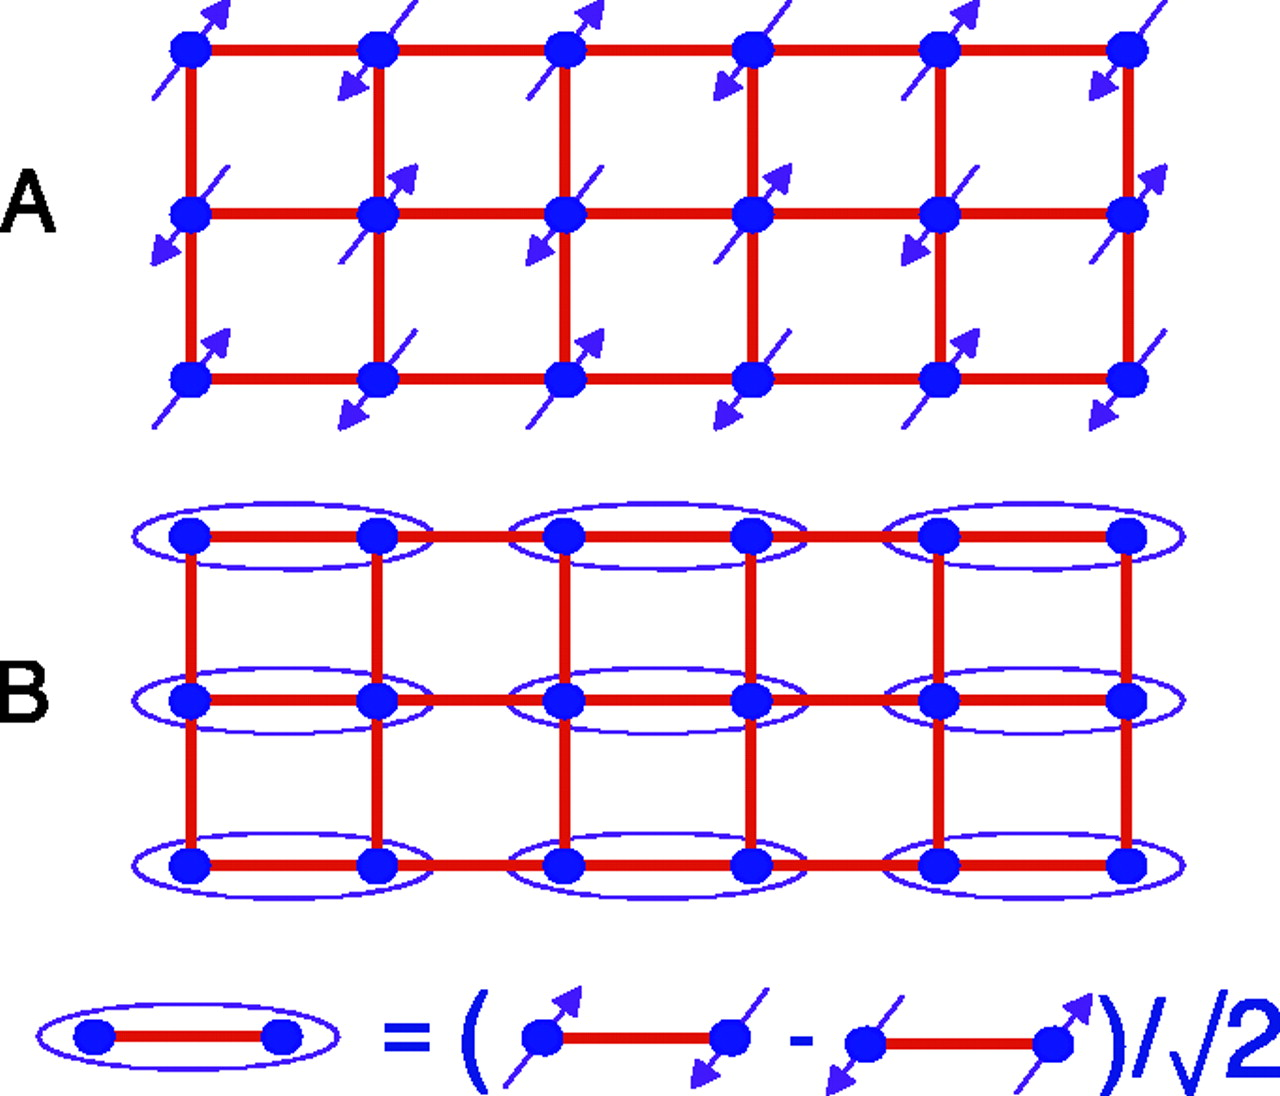
\includegraphics[width = 0.5\textwidth]{VBS Neel.jpeg}
        \caption{The VBS order breaks lattice translational symmetry while the N\'eel order breaks the O(3) rotational symmetry. After  T. Senthil \emph{et. al.}, \emph{Science} \textbf{303}, 1490 (2004)}
    \end{figure}
\end{frame}
%%%%%%%%%%%%%%%%%%%%%%%%%%%%%%%%%%%%%%%%%%%%%%%%
\begin{frame}{Deconfined Quantum Critical Point}
    \[\mathcal{H} = J\sum_{\anglelr{\bo{r}\bo{r}'}}\hat{\bo{S}}_{\bo{r}}\cdot\hat{\bo{S}}_{\bo{r}'} + \cdots\]
    \[\hat{\bo{n}} = z^\dagger\bog{\sigma}z\]
    \[\mathcal{L} = \sum_{\alpha=1}^{2}\abs{\lr{\de_{\mu}-i a_\mu}z_\alpha}^2 + s\abs{z}^2 + u\abs{z}^4 + \kappa\lr{\epsilon_{\mu\nu\kappa}\de_\nu a_\kappa}^2\]

{\tiny T. Senthil \emph{et. al.}, \emph{Science} \textbf{303}, 1490 (2004)}

\end{frame}
%%%%%%%%%%%%%%%%%%%%%%%%%%%%%%%%%%%%%%%%%%%%%%%%
\begin{frame}{$\mathrm{SrCu_2(BO_3)_2}$ and the Theoretical Model}
\subsection{$\mathrm{SrCu_2(BO_3)_2}$ and the Theoretical Model}
\begin{figure}
    \centering
    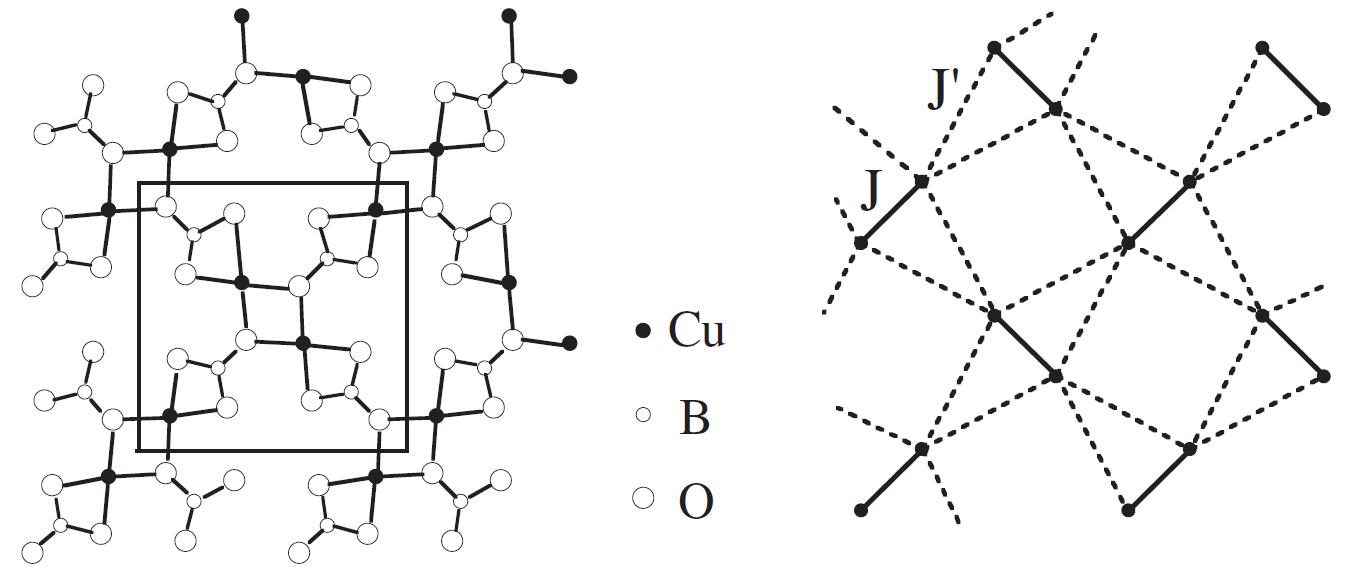
\includegraphics[width = 0.8\textwidth]{material illustration.png}
    \caption{Structure of the magnetic layer in $\mrm{SrCu_2(BO_3)_2}$. \\  K. Kodama \emph{et. al.}, \emph{J. Phys.: Condens. Matter} \textbf{14}, L319 (2002) }
\end{figure}
    
\end{frame}
%%%%%%%%%%%%%%%%%%%%%%%%%%%%%%%%%%%%%%%%%%%%%%%%
\begin{frame}{$\mathrm{SrCu_2(BO_3)_2}$ and the Theoretical Model}
\begin{itemize}
    \item \textbf{Shastry-Sutherland Model (SSM)}
\end{itemize}
\[\mathcal{H} = J\sum_{\anglelr{ij}}\hat{\bo{S}}_i\cdot\hat{\bo{S}}_j + J'\sum_{\anglelr{ij} \in \Box_s}\hat{\bo{S}}_i\cdot\hat{\bo{S}}_j - h\sum_{i}\hat{S}^z_i\]
\begin{figure}
    \centering
    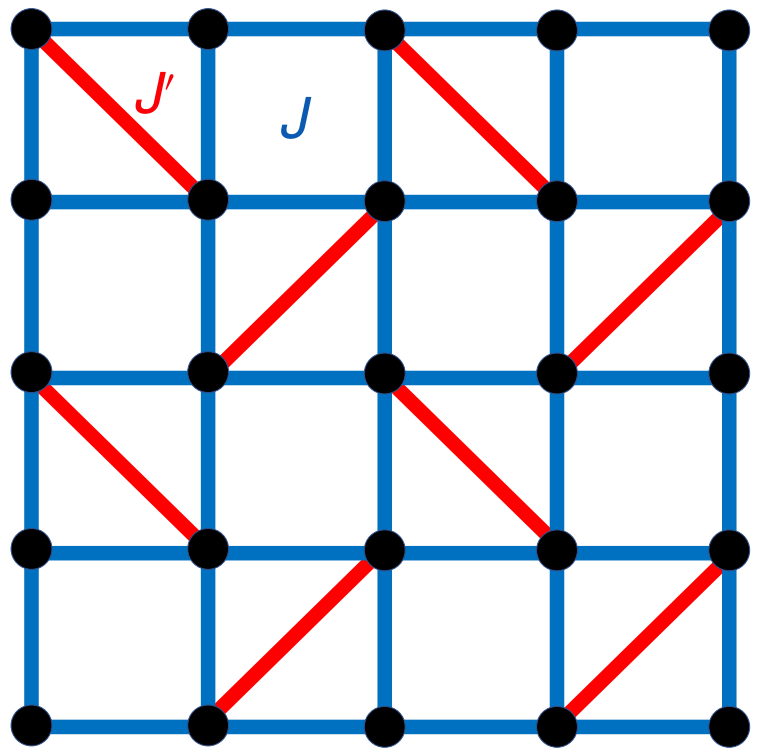
\includegraphics[width = 0.3\textwidth]{SSM.png}
    \caption{Shastry-Sutherland Model (SSM) on a square lattice. \emph{Nat. Phys.} \textbf{15}, 678 (2019)}
\end{figure}
    
\end{frame}
%%%%%%%%%%%%%%%%%%%%%%%%%%%%%%%%%%%%%%%%%%%%%%%%
\begin{frame}{$\mathrm{SrCu_2(BO_3)_2}$ and the Theoretical Model}
    \[\mathcal{H} = -J\sum_{\anglelr{ij}}P_{ij} - Q\sum_{ijkl\in \Box_s}\lr{P_{ij}P_{kl} + P_{ik}P_{jl}} - h\sum_{i}S^z_i\]
    \[P_{ij} = \frac{1}{4} - \hat{\bo{S}}_i\cdot\hat{\bo{S}}_j\]
    \begin{figure}
        \centering
        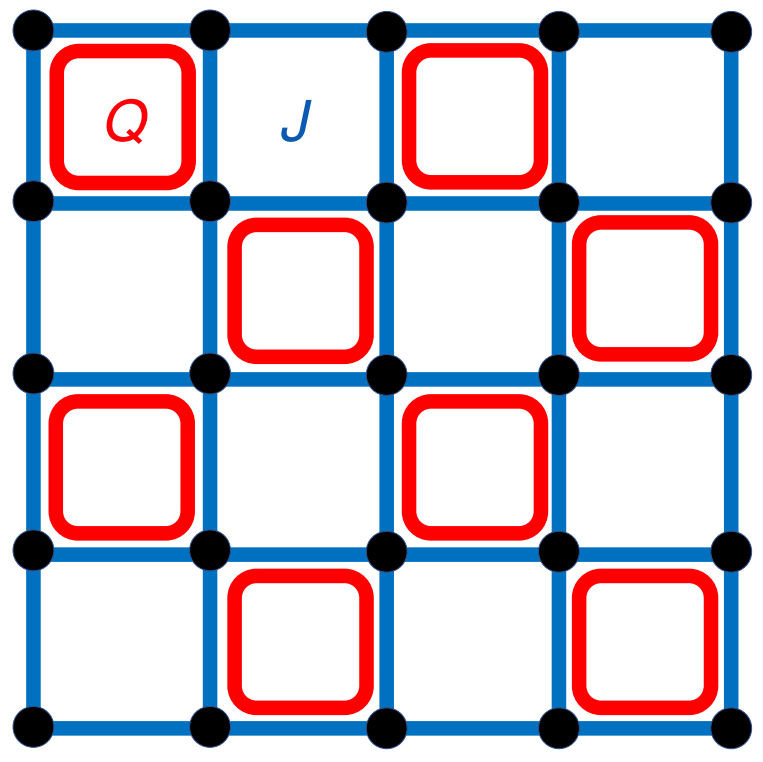
\includegraphics[width = 0.3\textwidth]{CBJQ.png}
        \caption{Checkerboard J-Q model. the $J'$ term is transformed effectively to the $Q$ term (4 spin coupling) here}
    \end{figure}
\end{frame}
%%%%%%%%%%%%%%%%%%%%%%%%%%%%%%%%%%%%%%%%%%%%%%%%
\begin{frame}{$\mathrm{SrCu_2(BO_3)_2}$ and the Theoretical Model}
    \begin{figure}
        \centering
        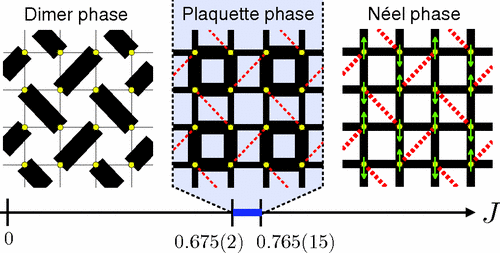
\includegraphics[width = 0.7\textwidth]{PS phase diagram.png}
        \caption{Three phases in the Shastry-Sutherland model (SSM) predicted numerically. \textit{Phys. Rev. B} \textbf{87}, 115144 (2013)}
    \end{figure}
\end{frame}
%%%%%%%%%%%%%%%%%%%%%%%%%%%%%%%%%%%%%%%%%%%%%%%%
\begin{frame}{About this Paper}
\subsection{About this Paper}
    \begin{itemize}
        \item To confirm the phase diagrom of $\mrm{SrCu_2(BO_3)_2}$ materials.

\vspace{0.5cm}
        
        \item Try to find the DQCP of the material $\mrm{SrCu_2(BO_3)_2}$ through nuclear magnetic resonance (NMR) method.

\vspace{0.5cm}
        
        \item Although they didn't find the DQCP actually, they pointed out the possibility of the existance of the DQCP and the possible future work to find it. 
    \end{itemize}
\end{frame}
%%%%%%%%%%%%%%%%%%%%%%%%%%%%%%%%%%%%%%%%%%%%%%%%
\begin{frame}{Phase Diagram Overview}
\subsection{Phase Diagram Overview}
    \begin{figure}
        \centering
        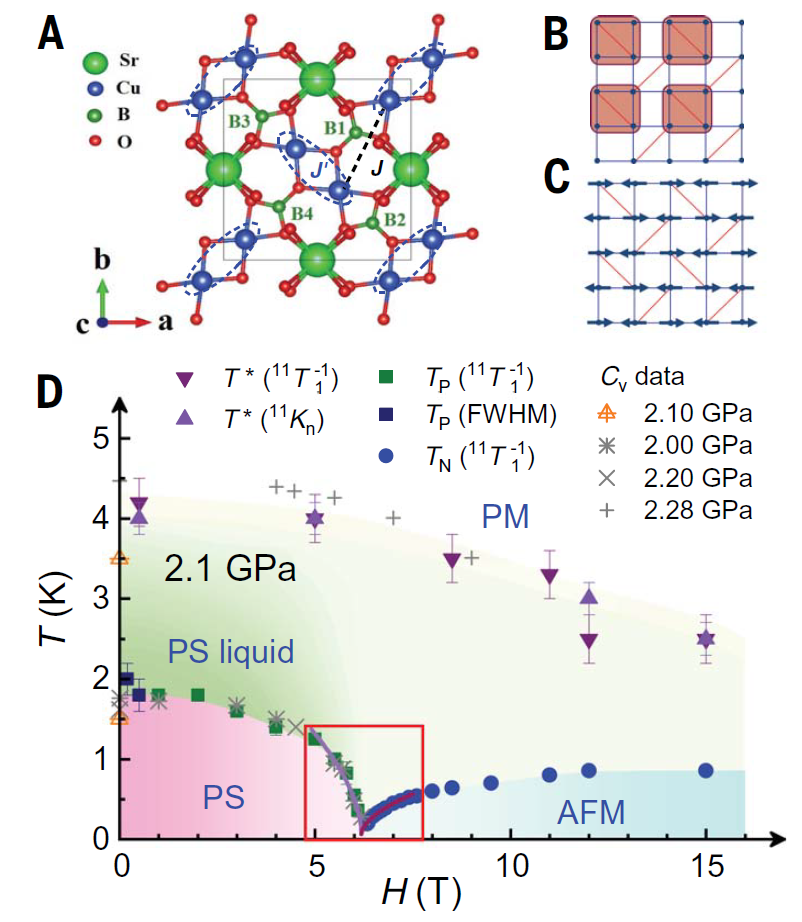
\includegraphics[width=0.5\textwidth]{phase.png}
        \caption{The phase diagram of $\mrm{SrCu_2(BO_3)_2}$ under pressure 2.1GPa}
    \end{figure}
    
    % Three phases: (i) plaquette singlet (ii) AFM (iii) plaquette singlet liquid.
\end{frame}
%%%%%%%%%%%%%%%%%%%%%%%%%%%%%%%%%%%%%%%%%%%%%%%%
\begin{frame}{Phase Diagram Overview}
    \begin{figure}
        \centering
        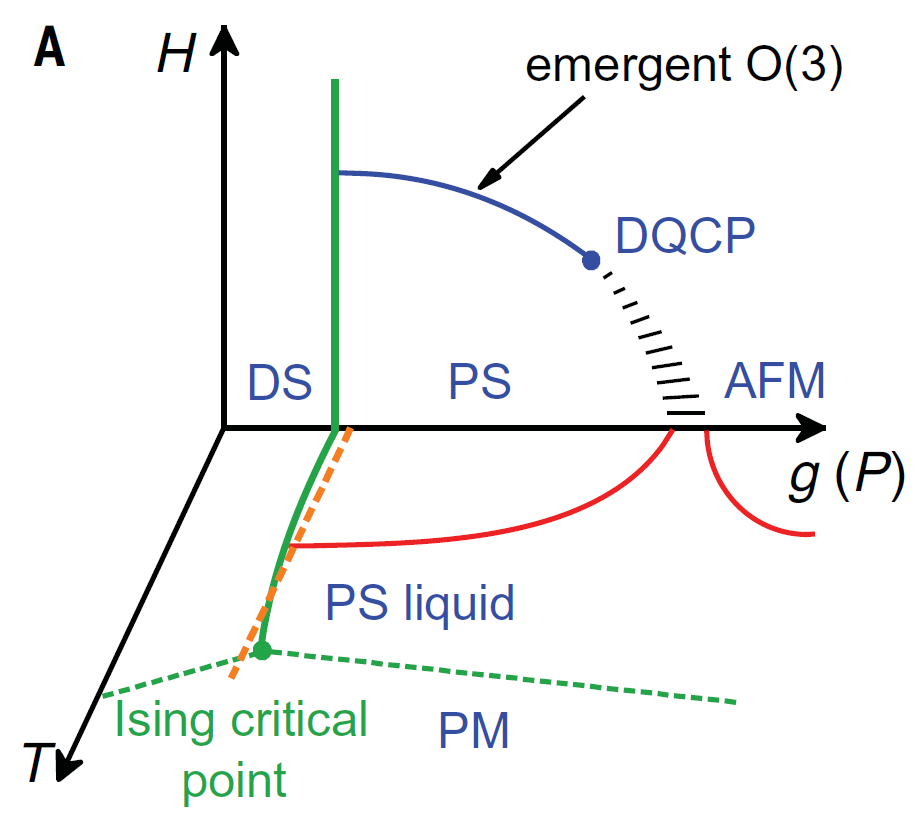
\includegraphics[height = 0.55\textheight]{3phase1.png}
        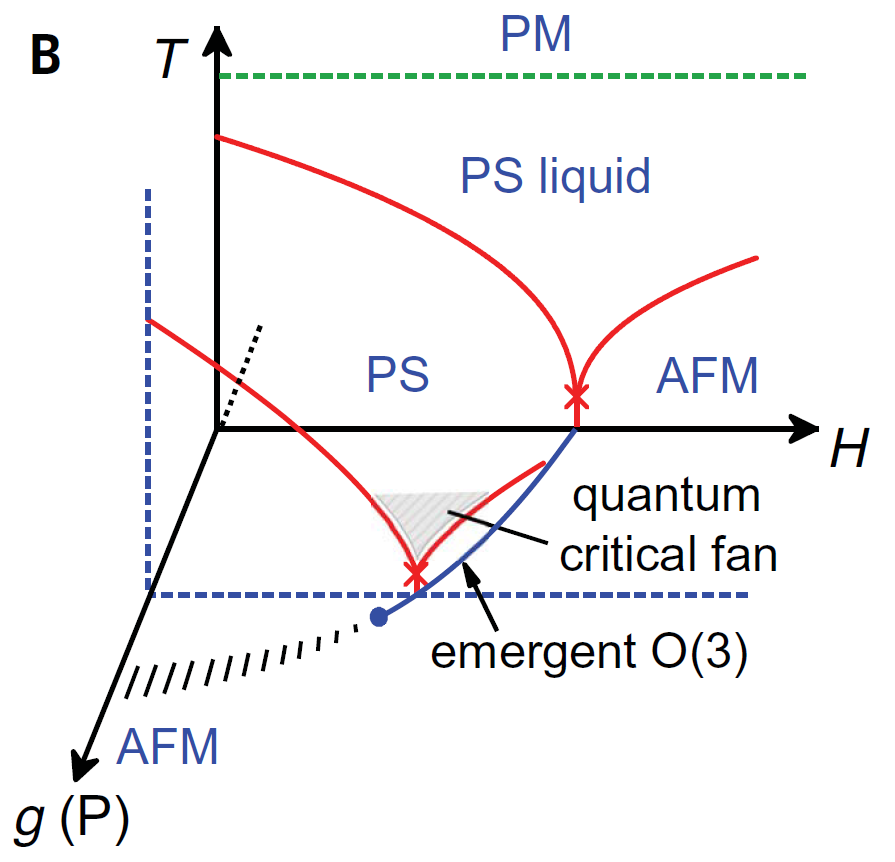
\includegraphics[height = 0.55\textheight]{3phase2.png}
        \caption{There are three parameters can be tuned. They are (i) \alert{temperature}, (ii) external \alert{magnetic field}, and (iii) \alert{pressure}. Where the pressure can change the value of $J'/J$ in the SSM.}
    \end{figure}

    % The DQCP is predicted, they didn't confirm its existance in this experiment actually. However they indeed find an important effect that implies the existance of the DQCP. That is, the first order feature is weaken as the pressure increases.

    % The goal of this paper is to characterize the FIELD DRIVEN PS-AFM TRANSISION.
    
\end{frame}
%%%%%%%%%%%%%%%%%%%%%%%%%%%%%%%%%%%%%%%%%%%%%%%%
{
\setbeamercolor{background canvas}{bg=lightgray}
\section{Experimental Method}
\begin{frame}
    \centering
    \huge
    \textbf{Experimental Method}
\end{frame}
}
%%%%%%%%%%%%%%%%%%%%%%%%%%%%%%%%%%%%%%%%%%%%%%%%
\begin{frame}{NMR Spectrum}
\subsection{NMR spectrum}
    The authors performed a $^{11}\mrm{B}$ NMR measurement
    \begin{figure}
        \centering
        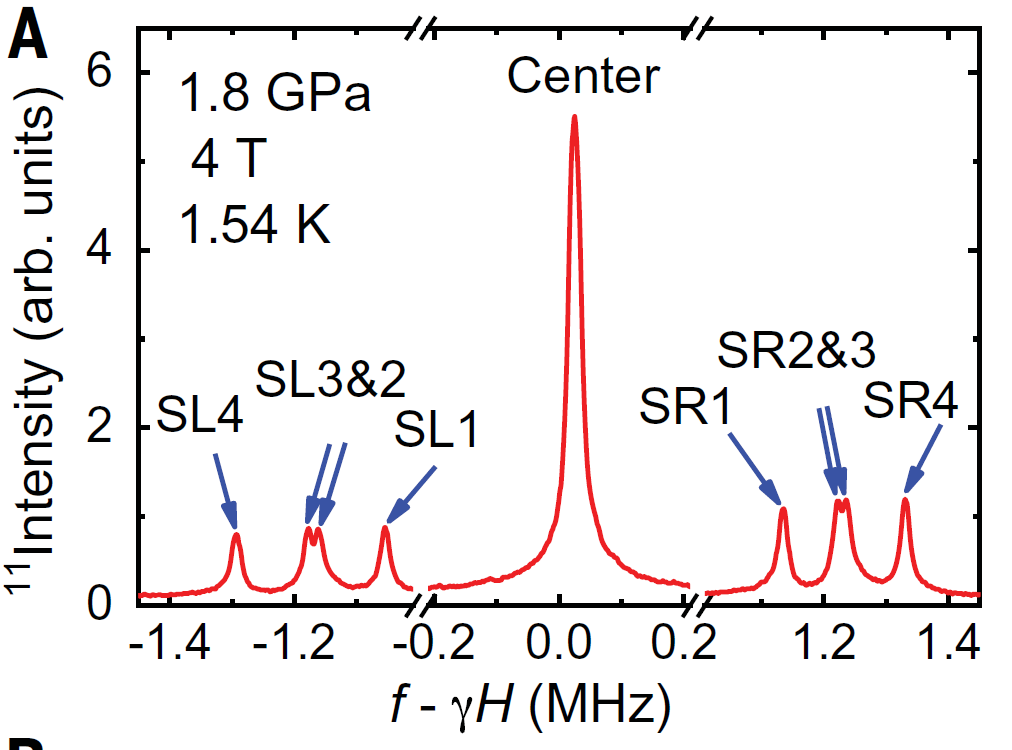
\includegraphics[height = 0.4\textheight]{general spectrum.png}
        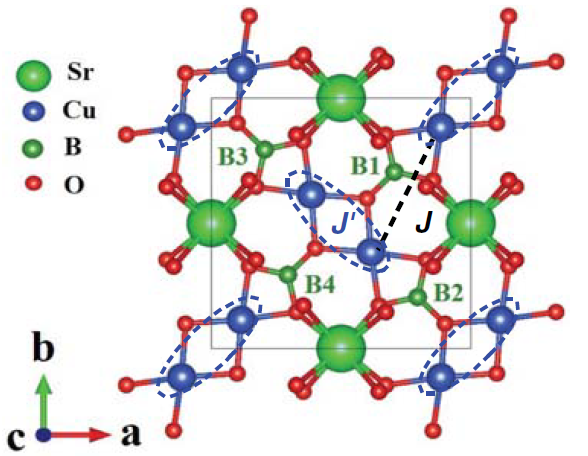
\includegraphics[height = 0.4\textheight]{structure.png}
        \caption{(Left) the $^{11}\mrm{B}$ NMR spectrum, including a central line and few satellite peaks arises from different positions of boron ions (right)}
    \end{figure}

    % Investigating the Kight shift and the spectral line splitting can let us know the information of the phases.

    % "Spins" in the spin model is carried by Cu ions. The arrangement of Cu spins (corresponding to different phases) will affect the boron NMR spectrum due to the hyperfine interaction.
    
\end{frame}
%%%%%%%%%%%%%%%%%%%%%%%%%%%%%%%%%%%%%%%%%%%%%%%%
\begin{frame}{NMR Spectrum}
    \begin{figure}
        \centering
        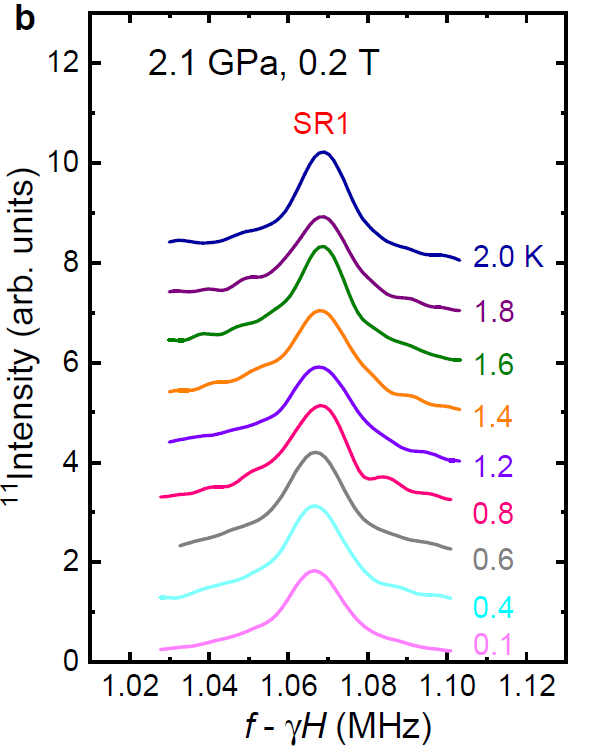
\includegraphics[height = 0.55\textheight]{broaden peaks.png}
        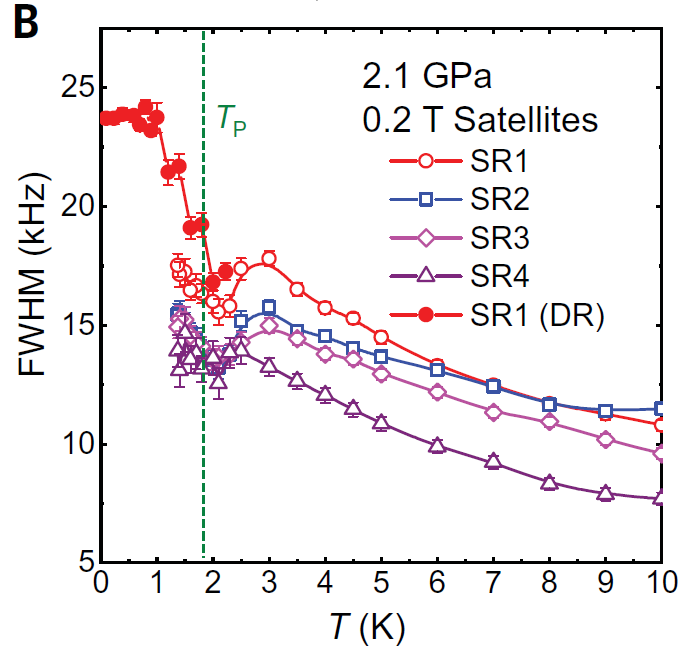
\includegraphics[height = 0.55\textheight]{3B.png}
        \caption{Full width at half maximum (FWHM) of each satellite peak at different temperature. The sharp inclination indicates the \alert{formation of plaquette singlet (PS) } phase. }
    \end{figure}
\end{frame}
%%%%%%%%%%%%%%%%%%%%%%%%%%%%%%%%%%%%%%%%%%%%%%%%
\begin{frame}{NMR Spectrum}
    \begin{figure}
        \centering
        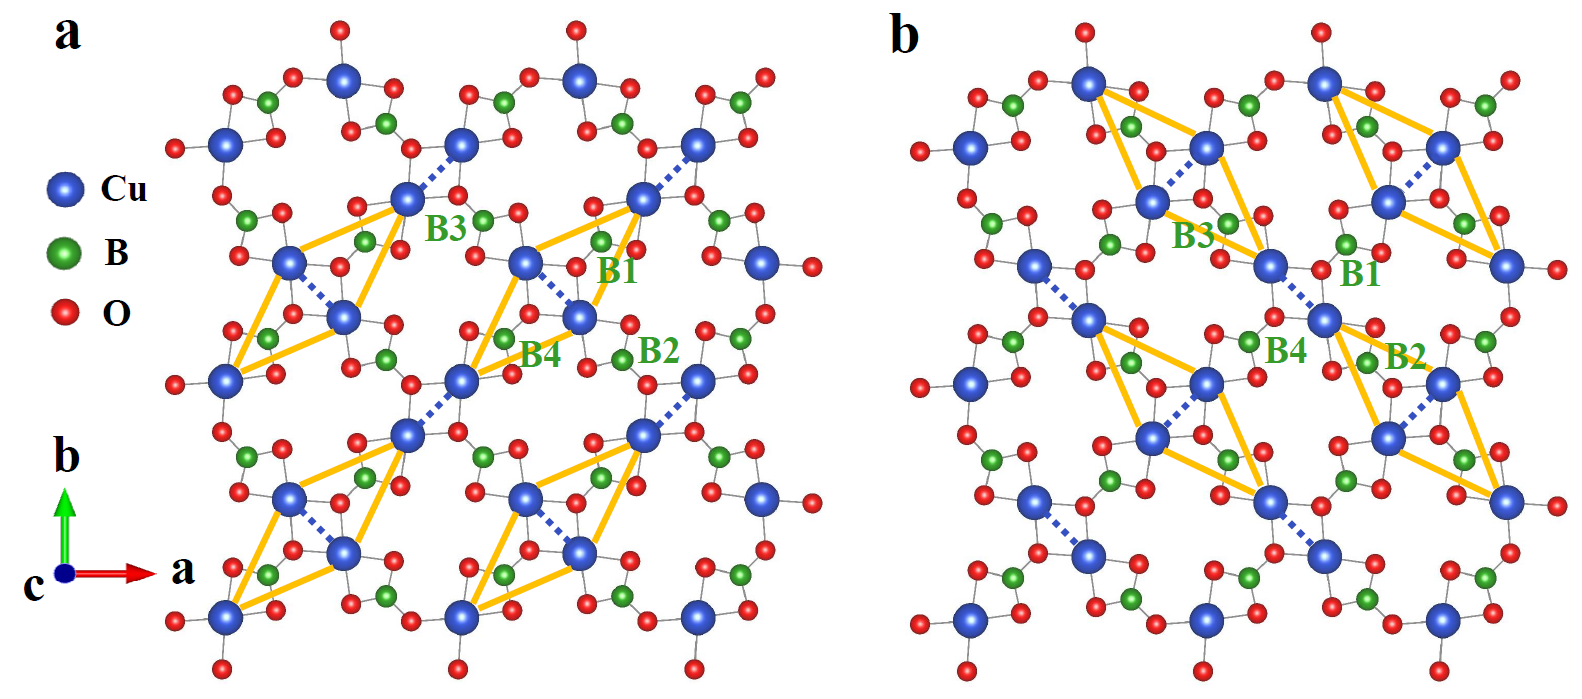
\includegraphics[width = 0.7\textwidth]{PS forming and line width broadening.png}
        \caption{PS order formation leads to the lattice distortion, which broaden the satellite line width.}
    \end{figure}
\end{frame}
%%%%%%%%%%%%%%%%%%%%%%%%%%%%%%%%%%%%%%%%%%%%%%%%
\begin{frame}{NMR Spectrum}
Applying an \textbf{external magnetic field} (parallel to $c$-axis) induces central line splitting. Three peaks indicating the PS \& AFM phase coexistence. 
    \begin{figure}
        \centering
        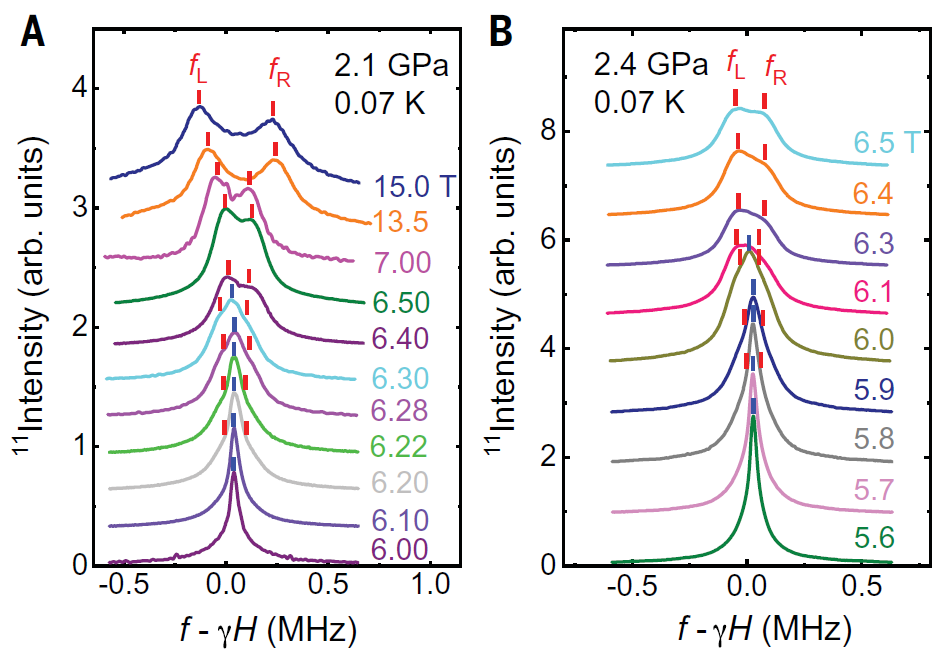
\includegraphics[width = 0.6\textwidth]{magnetic induced line splitting.png}
        \caption{Field induced line splitting under pressure 2.1 GPa and 2.4 GPa respectively.}
    \end{figure}
\end{frame}
%%%%%%%%%%%%%%%%%%%%%%%%%%%%%%%%%%%%%%%%%%%%%%%%
\begin{frame}{NMR Spectrum}
    \begin{figure}
        \centering
        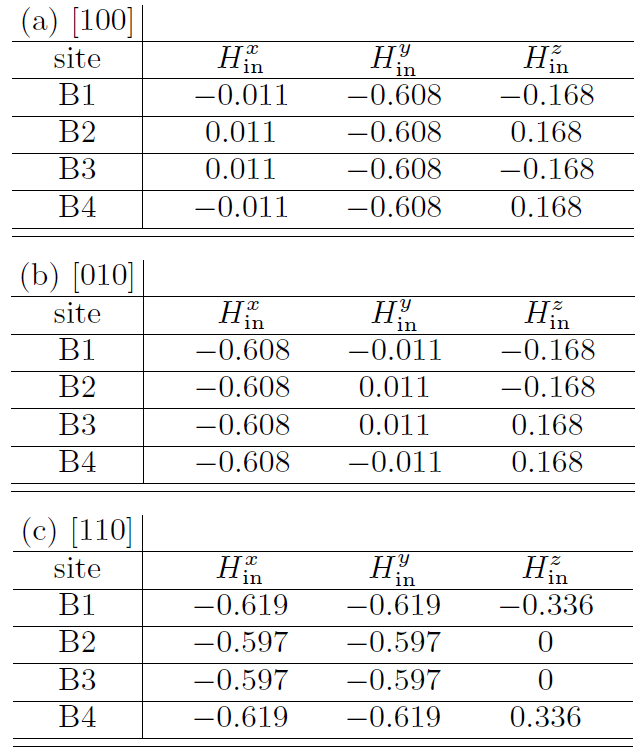
\includegraphics[height = 0.6\textheight]{hyperfine table.png}
        \caption{The \textbf{hyperfine field} at each boron ion sites. }
    \end{figure}
\end{frame}
%%%%%%%%%%%%%%%%%%%%%%%%%%%%%%%%%%%%%%%%%%%%%%%%
\begin{frame}{Relaxation Rate}
\subsection{Relaxation Rate}
    The \textbf{spin-lattice relaxation rate} is a direct indicator of the low energy \textbf{spin fluctuation} (hence related to the magnetic susceptibility).
    \[\frac{1}{T_1} \propto \frac{T}{\mu_B^2}\lim_{\omega\to 0}\sum_{\bo{q}}F_{\alpha}\lr{\bo{q}}\frac{\chi''\lr{\bo{q},\omega}}{\omega}\]

    $1/T_1$ and $\chi$ (spin fluctuation) are related through the \textbf{spin hyperfine interaction} 

    \vspace{0.5cm}

    $1/T_1$ is a good indicator to clearly show the \textbf{PS-AFM} phase transition.

    % Brefly introduce the definition of the relaxation rate.
\end{frame}
%%%%%%%%%%%%%%%%%%%%%%%%%%%%%%%%%%%%%%%%%%%%%%%%
\begin{frame}{Relaxation Rate}
    \begin{figure}
        \centering
        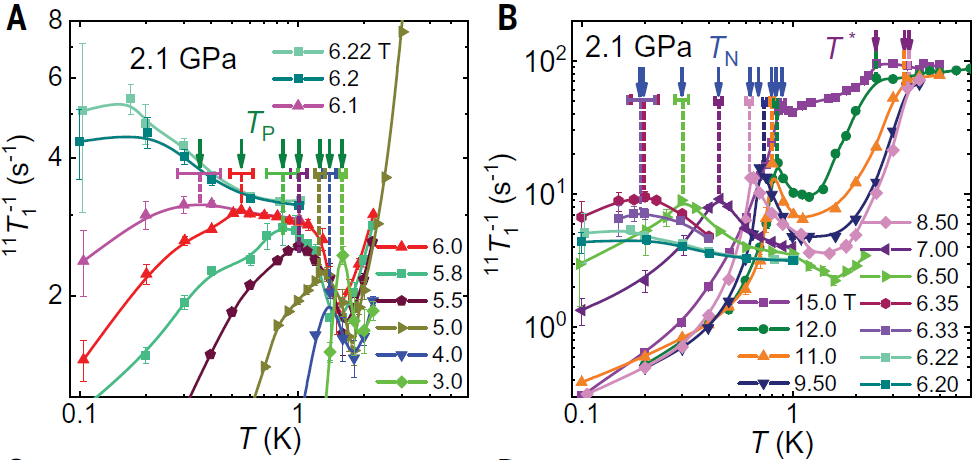
\includegraphics[width = 0.7\textwidth]{rate phase transition.png}
        \caption{Temperature induced phase transitions under different magnetic field. (Left) A PS-PS liquid transition. (Right) An AFM-PS liquid transition.}

        % A rapid drop of $1/T_1$ in the PS-PS liquid transition (into the PS phase) arises from the existance of SPIN GAP \Delta. (PS phase is a gapped phase, and notice that AFM is a gapless phase)

        
    \end{figure}
\end{frame}
%%%%%%%%%%%%%%%%%%%%%%%%%%%%%%%%%%%%%%%%%%%%%%%%
{
\setbeamercolor{background canvas}{bg=lightgray}
\section{Discussion}
\begin{frame}
    \centering
    \huge
    \textbf{Discussion}
\end{frame}
}
%%%%%%%%%%%%%%%%%%%%%%%%%%%%%%%%%%%%%%%%%%%%%%%%
\begin{frame}{Weaken Discontinuity}
\subsection{Weaken Discontinuity}
Under a higher pressure, the discontinuity in $(f_R-f_L)$ is weaken, indicating a weak first-order transition.
    \begin{figure}
        \centering
        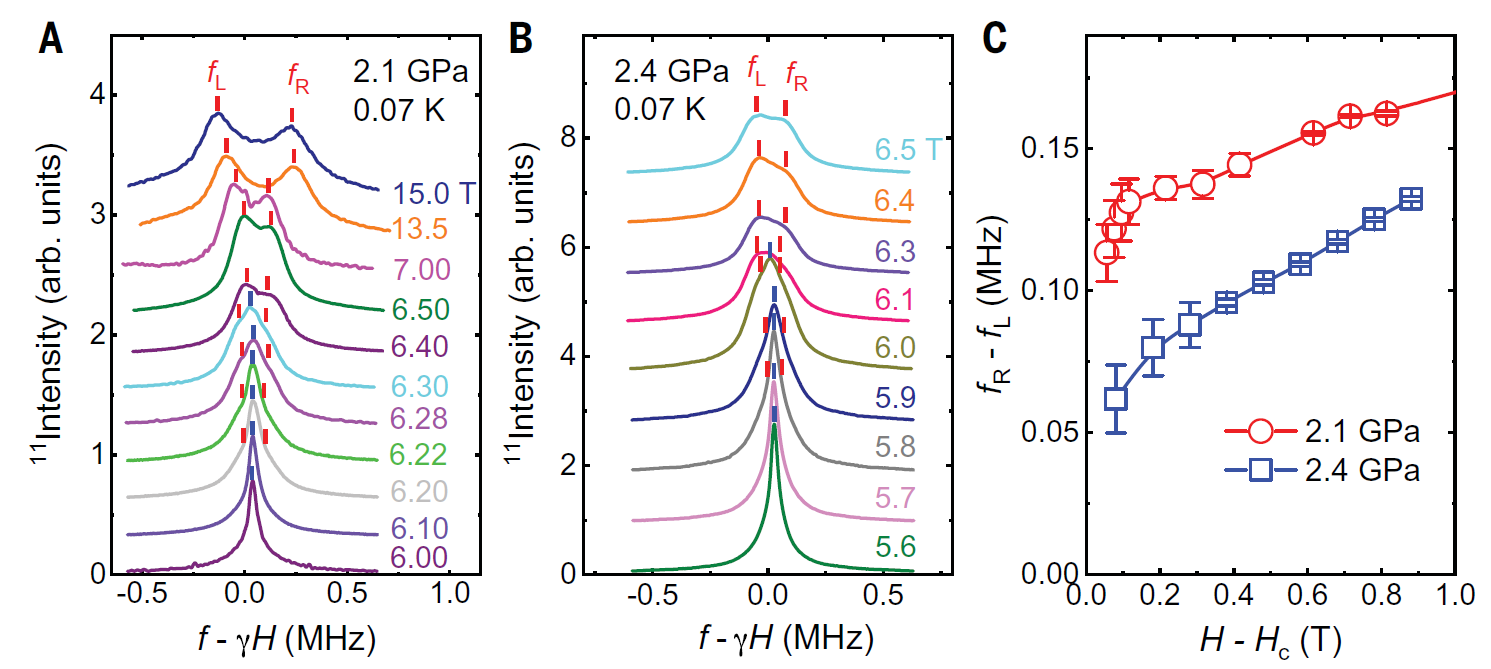
\includegraphics[width = 0.8\textwidth]{AFM splitting.png}
        \caption{Field induced line splitting. The discontinuity in $(f_R-f_L)$ shows that the phase transition is first order.}
    \end{figure}
\end{frame}
%%%%%%%%%%%%%%%%%%%%%%%%%%%%%%%%%%%%%%%%%%%%%%%%
\begin{frame}{Weaken Discontinuity}
Scaling behaviour appears under a higher pressure (2.4 GPa)
\[\chi \propto 1/T_1 \sim aT^{\eta}\]
    \begin{figure}
        \centering
        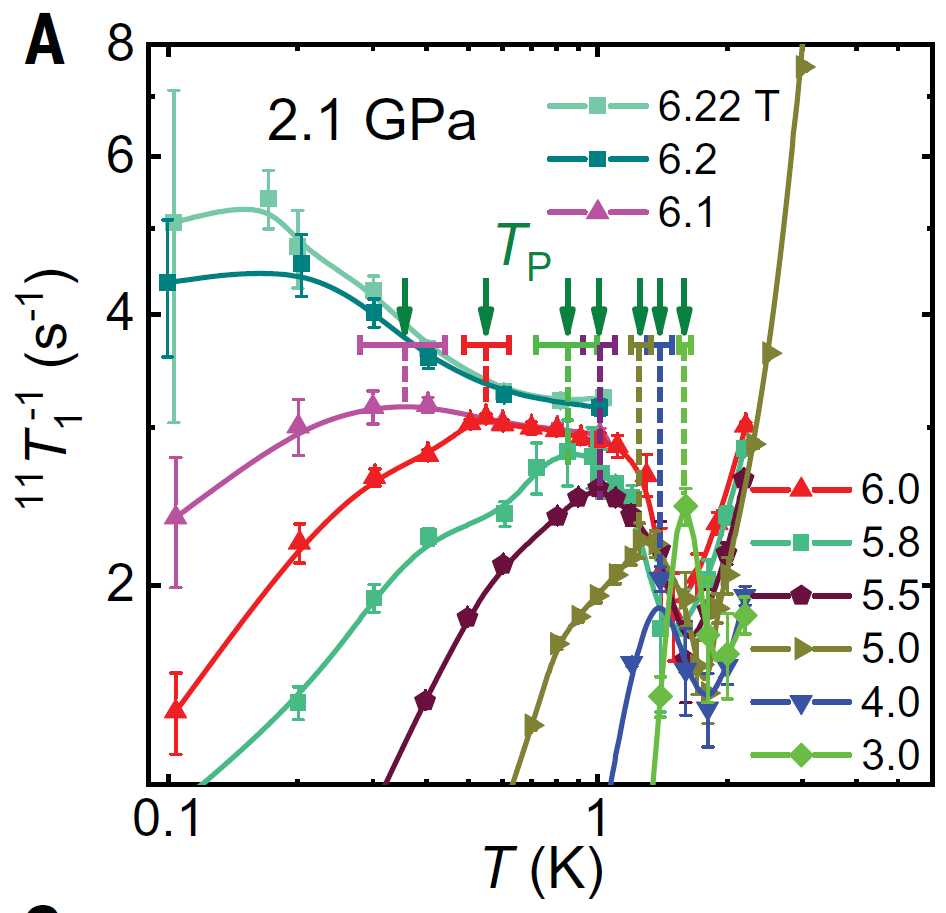
\includegraphics[height = 0.45\textheight]{5A.png}
        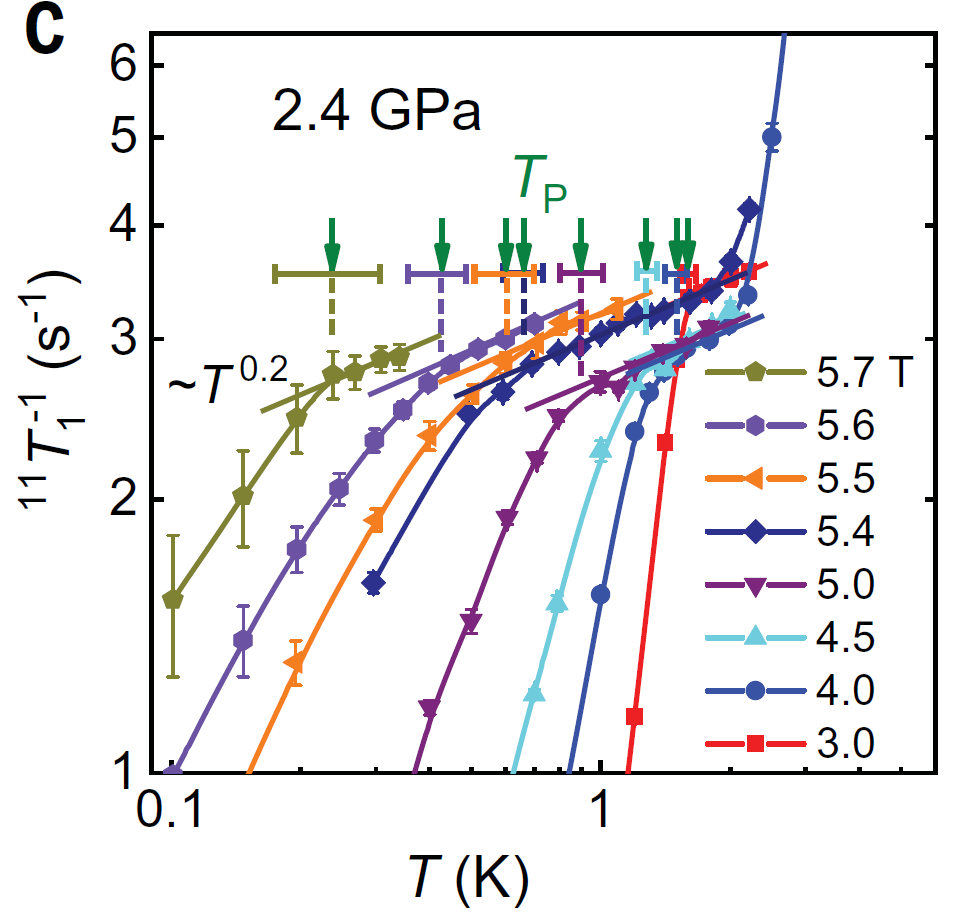
\includegraphics[height = 0.45\textheight]{5c.png}
        \caption{temperature induced phase transition with $1/T_1$ as the indicator.}
    \end{figure}
\end{frame}
%%%%%%%%%%%%%%%%%%%%%%%%%%%%%%%%%%%%%%%%%%%%%%%%
\begin{frame}{Numerical Simulation of J-Q Model}
\subsection{Numerical Simulation of J-Q Model}
Another important concept about DQCP is the \textbf{emergent  symmetry}.  

\vspace{0.3cm}

The authors applied quantum Monte Carlo method to showed that emergent symmetry of the \textbf{J-Q model in a magnetic field} is $O(3)$. 

\[m_p = \frac{1}{L^2/2}\sum_{i\in\Box_s}(-1)^{i_x}S^z(i)S^z(i+\hat{\bo{x}})S^z(i+\hat{\bo{y}})S^z(i+\hat{\bo{x}} + \hat{\bo{y}})\]
Emergent order parameter:
\[(m_x,m_y)\otimes m_p \to (m_x,m_y,m_p)\]
the combination becomes a $O(3)$ vector, corresponding to an $O(3)$ non-linear sigma model.


\end{frame}
%%%%%%%%%%%%%%%%%%%%%%%%%%%%%%%%%%%%%%%%%%%%%%%%
\begin{frame}{Numerical Simulation of J-Q Model}
In the presence of $O(3)$ symmetry, the probability distribution of $m_p$ should be uniform (like a flat plateau).
    \begin{figure}
        \centering
        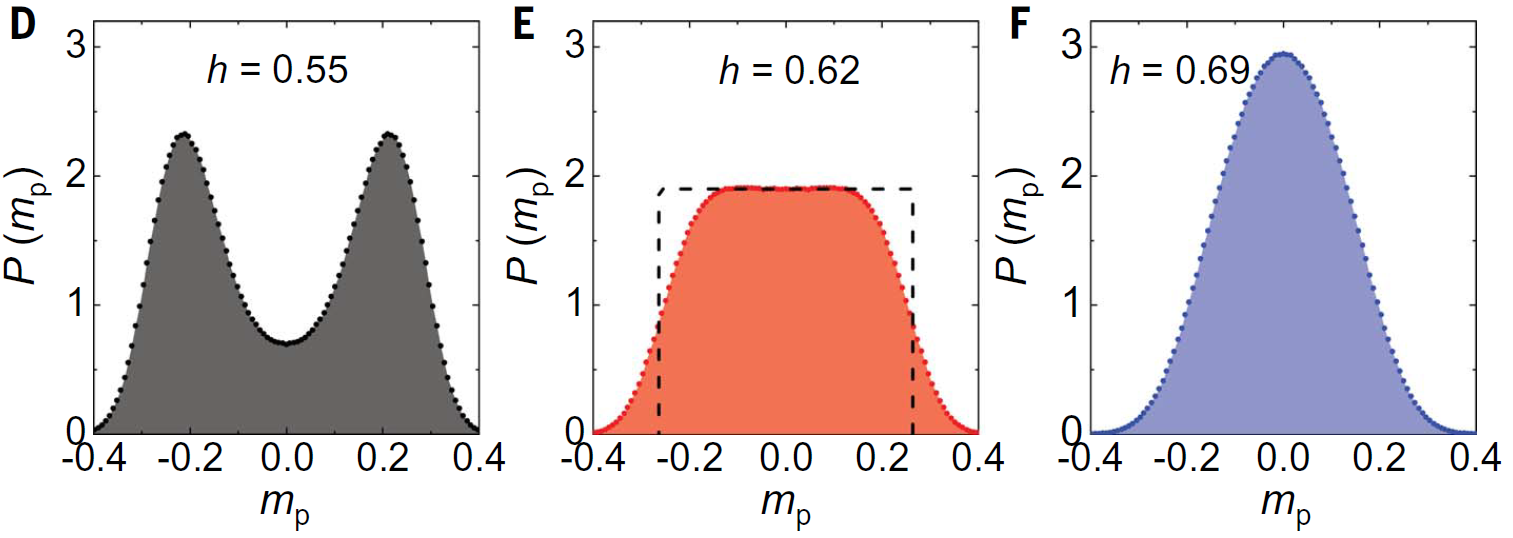
\includegraphics[width = 0.8\textwidth]{simulation.png}
        \caption{(Left) PS phase, Ising-like symmetry. (Middle) DQCP,  emergent O(3). (Right) AFM phase (no PS order, thus the avarage value is zero).}
    \end{figure}
So the numerical result suggest an emergent $O(3)$ symmetry.
\end{frame}
%%%%%%%%%%%%%%%%%%%%%%%%%%%%%%%%%%%%%%%%%%%%%%%%
\begin{frame}{Outlook}
\subsection{Outlook}
    \begin{itemize}
        \item To further increase the pressure to see if there indeed exist a DQCP. 

        \item Identify the fractional excitations and the emerged gauge field.
    \end{itemize}
\end{frame}
%%%%%%%%%%%%%%%%%%%%%%%%%%%%%%%%%%%%%%%%%%%%%%%%
\begin{frame}
    \centering
\Huge
\textsc{Thanks for Listening}
\end{frame}
%%%%%%%%%%%%%%%%%%%%%%%%%%%%%%%%%%%%%%%%%%%%%%%%
%%%%%%%%%%%%%%% Supplement %%%%%%%%%%%%%%%%%%%%%
%%%%%%%%%%%%%%%%%%%%%%%%%%%%%%%%%%%%%%%%%%%%%%%%
\begin{frame}{Supplement-Knight Shift}
    \textbf{Knight Shift} here indicates the changing of magnetic susceptibility $\chi$.
    \[K_{ii} = \mu_B N_A \chi A_{ii} \]
    where $\bo{A}$ is the hyperfine interaction tensor
    \[H_{i} = A_{ij}m_j\]
{\tiny K. Kodama \textit{et. al}., \textit{J. Phys.: Condens. Matter} \textbf{14}, L319 (2002)}
\end{frame}
%%%%%%%%%%%%%%%%%%%%%%%%%%%%%%%%%%%%%%%%%%%%%%%%
\begin{frame}{Supplement-Knight Shift}
    \begin{figure}
        \centering
        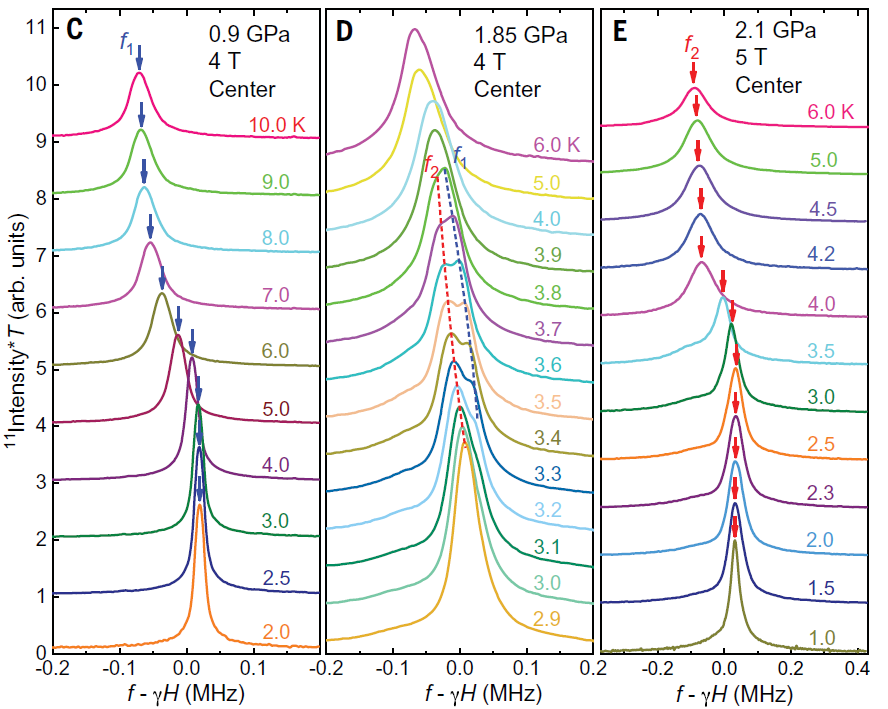
\includegraphics[width = 0.6\textwidth]{knight shift DS PS transition.png}
        \caption{(Left) Central peaks in the DS phase. (Middle) DS and PS phase coexistence. (Right) Central peaks in the PS phase. The rapid change of the Knight shift in the right penal indicates a PS-PS liquid transition. }
    \end{figure}
\end{frame}
%%%%%%%%%%%%%%%%%%%%%%%%%%%%%%%%%%%%%%%%%%%%%%%%
\begin{frame}{Supplement-Other Numerical Simulation}
\small Another research indicated (using quantum Monte Carlo method) the emergent enhanced symmetry is $O(4)$ by plotting the probability $P(m_z, m_p)$ where $m_p$ is the PS order parameter.

Notice that the system here is not under a magnetic field. The magnetic field, as shown in the main paper, breaks the original $O(3)$ N\'eel order parameter to $O(2)$, therefore the final dimension enlarged order parameter is $\lr{m_x,m_y,m_p}$, which possesses an emergent $O(3)$ symmetry.  
    \begin{figure}
        \centering
        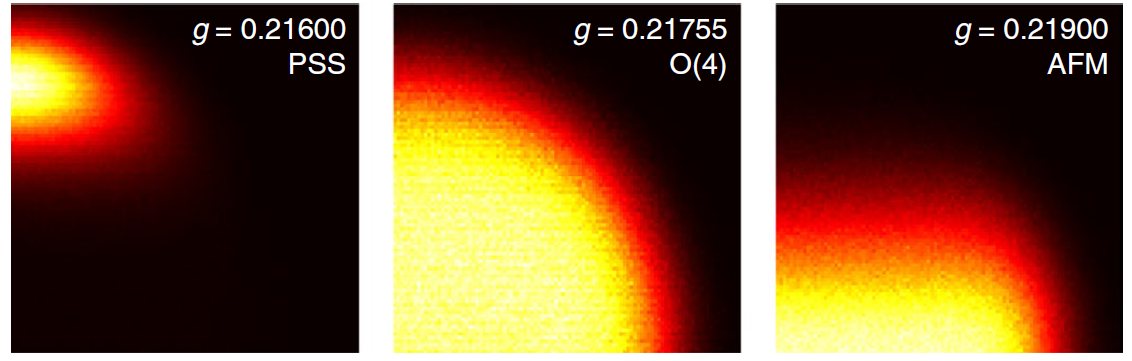
\includegraphics[width = 0.7\textwidth]{O4 symmetry.png}
        \caption{A numerical result confirmed the emergent $O(4)$ symmetry. \textit{Nat. Phys.} \textbf{15}, 678 (2019)}
    \end{figure}
    


\end{frame}
%%%%%%%%%%%%%%%%%%%%%%%%%%%%%%%%%%%%%%%%%%%%%%%%
\begin{frame}{Supplement-Spin Gap}
The spin-lattice relaxation rate possesses the following relation with temperature
    \[\frac{1}{T_1} \propto T^\alpha e^{-\Delta/k_B T}\]
where $\Delta$ is the spin gap.

There will be a sharp drop of the \textbf{relaxation rate} (which is actually proportional to the \textbf{spin fluctuation}, hence be proportional to the \textbf{magnetic susceptibility $\chi$}) because of the existence of the gap.  
\end{frame}
%%%%%%%%%%%%%%%%%%%%%%%%%%%%%%%%%%%%%%%%%%%%%%%%
\end{document}

